\documentclass[12pt]{article}
\usepackage[paper=letterpaper,margin=2cm]{geometry}
\usepackage{amsmath,amssymb,amsfonts}
\usepackage{newtxtext, newtxmath}
\usepackage{enumitem}
\usepackage{titling}
\usepackage[colorlinks=true]{hyperref}
\usepackage{multirow}
\usepackage{svg}
\usepackage{listings}
\usepackage{xcolor}
\usepackage{float}

\setlength{\droptitle}{-6em}

\definecolor{codegreen}{rgb}{0,0.6,0}
\definecolor{codegray}{rgb}{0.5,0.5,0.5}
\definecolor{codepurple}{rgb}{0.58,0,0.82}
\definecolor{backcolour}{rgb}{0.95,0.95,0.92}

\lstdefinestyle{mystyle}{
    commentstyle=\color{codegreen},
    keywordstyle=\color{magenta},
    numberstyle=\tiny\color{codegray},
    stringstyle=\color{codepurple},
    basicstyle=\ttfamily\footnotesize,
    breakatwhitespace=false,
    breaklines=true,
    captionpos=b,
    keepspaces=true,
    numbers=left,
    numbersep=5pt,
    showspaces=false,
    showstringspaces=false,
    showtabs=false,
    tabsize=2
}
\lstset{style=mystyle}

\begin{document}

\begin{center}
\large{Aprendizagem 2023}\\
Homework I -- Group 28\\
\vskip 0.3cm
Gonçalo Bárias (ist1103124) \& Raquel Braunschweig (ist1102624)\vskip 1cm

\large{\textbf{Part I}: Pen and Paper}\normalsize
\end{center}

\noindent Consider the partially learnt decision tree from the dataset $D$. $D$ is described by four input variables –
one numeric with values in $[0,1]$ and 3 categorical – and a target variable with three classes.

\begin{figure}[H]
    \centering
    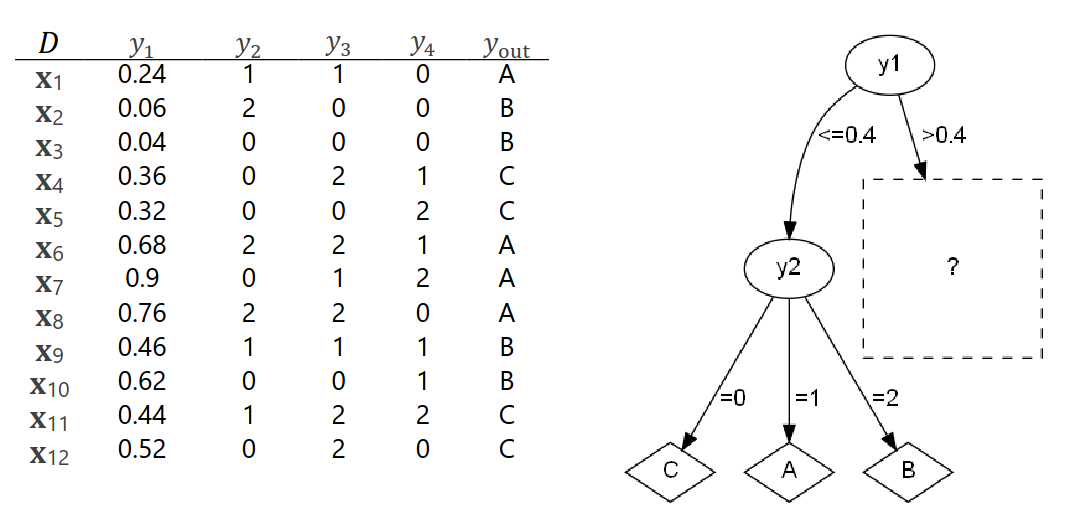
\includegraphics[width=15cm]{./assets/partial_tree_dataset_d}
    \caption{Partially Learnt Decision Tree and Dataset $D$ from Part I}
    \label{fig:PartI-partial-decision-tree-dataset-d}
\end{figure}

\begin{enumerate}[leftmargin=\labelsep]
    \item \textbf{Complete the given decision tree using Information gain with Shannon entropy ($log_2$).
    Consider that: i) a minimum of 4 observations is required to split an internal node, and
    ii) decisions by ascending alphabetic order should be placed in case of ties.}

    \vskip 0.3cm
    The entropy of \(y_{out}\) is given by:

    \begin{equation}
        \begin{split}
            E(y_{out} |y_1 > 0.4) = \quad
            & \quad  p(\text{A}, y_1 > 0.4) \log_2 \left(p(\text{A}, y_1 > 0.4)\right)  \\
            & + p(\text{B}, y_1 > 0.4) \log_2 \left(p(\text{B}, y_1 > 0.4)\right) \\
            & + p(\text{C}, y_1 > 0.4) \log_2 \left(p(\text{C}, y_1 > 0.4)\right) \\
        \end{split}
    \end{equation}

    We can calculate $E(y_{out})$:

    \[
        \begin{aligned}
            E(y_{out}) & = - \left(\frac{3}{7} \log_2\left(\frac{3}{7}\right) + \frac{2}{7} \log_2\left(\frac{2}{7}\right)
                            + \frac{2}{7} \log_2\left(\frac{2}{7}\right)\right) = 1.5567
        \end{aligned}
    \]

    The next step is calculating $E(y_{out} | y_1 > 0.4 , y_x)$, in which x will take the values of 2, 3 or 4:

    \begin{equation}\label{exI1-e-yout-y2}
        \begin{split}
            E(y_{out} |y_1 > 0.4 , y_x) = \quad
            & \quad  p(y_x = 0) E(y_{out} | y_x > 0.4 , y_2 = 0) \\
            & + p(y_x = 1) E(y_{out} | y_x > 0.4 , y_2 = 1) \\
            & + p(y_x = 2) E(y_{out} | y_x > 0.4 , y_2 = 2)
        \end{split}
    \end{equation}

    And the information gain of variable $y_x$ is given by

    \begin{equation}\label{ex1-ig}
        IG(y_x) = E(y_{out}) - E(y_{out} |y_1 > 0.4, y_x)
    \end{equation}

    \textbf{Let's start with x = 2}:

    \[
        \begin{aligned}
            p(y_2 = 0, y_1 > 0.4)          & = \frac{3}{7}                                                                                               \\
            p(y_2 = 1, y_1 > 0.4)          & = \frac{2}{7}                                                                                              \\
            p(y_2 = 1, y_1 > 0.4)          & = \frac{2}{7}                                                                                              \\
            E(y_{out} | y_x > 0.4 , y_2 = 0) & = - \left(\frac{1}{3} \log_2\left(\frac{1}{3}\right) + \frac{1}{3} \log_2\left(\frac{1}{3}\right)
                + \frac{1}{3} \log_2\left(\frac{1}{3}\right)\right) = 1.5849                                                                   \\
            E(y_{out} | y_x > 0.4 , y_2 = 1) & = - \left(\frac{0}{2} \log_2\left(\frac{0}{2}\right) + \frac{1}{2} \log_2\left(\frac{1}{2}\right)
                + \frac{1}{2} \log_2\left(\frac{1}{2}\right)\right) = 1                                                                        \\
            E(y_{out} | y_x > 0.4 , y_2 = 2) & = - \left(\frac{2}{2} \log_2\left(\frac{2}{2}\right) + \frac{0}{2} \log_2\left(\frac{0}{2}\right)
                + \frac{0}{2} \log_2\left(\frac{0}{2}\right)\right) = 0
        \end{aligned}
    \]

    Therefore, replacing these values on equation \eqref{exI1-e-yout-y2}, gives us:

    \[
        \begin{aligned}
            E(y_{out} | y_1>0.4, y_2) & = \frac{3}{7} \times 1.5849 + \frac{2}{7} \times 1 +  \frac{2}{7} \times 0 & = 0.965.
        \end{aligned}
    \]

    Finally, we can calculate the information gain, as per \eqref{ex1-ig},

    \[
        IG(y_{2}) = 1.5567 - 0.965 = 0.5917
    \]

    \textbf{Now, let's calculate for x = 3}:

    \[
        \begin{aligned}
            p(y_3 = 0, y_1 > 0.4)          & = \frac{1}{7}                                                                                    \\
            p(y_3 = 1, y_1 > 0.4)          & = \frac{2}{7}                                                                                    \\
            p(y_3 = 2, y_1 > 0.4)          & = \frac{4}{7}                                                                                    \\
            E(y_{out} | y_x > 0.4 , y_3 = 0) & = - \left(\frac{0}{1} \log_2\left(\frac{0}{1}\right) + \frac{1}{1} \log_2\left(\frac{1}{1}\right)
                + \frac{0}{1} \log_2\left(\frac{0}{1}\right)\right) = 0                                                                       \\
            E(y_{out} | y_x > 0.4 , y_3 = 1) & = - \left(\frac{1}{2} \log_2\left(\frac{1}{2}\right) + \frac{1}{2} \log_2\left(\frac{1}{2}\right)
                + \frac{0}{2} \log_2\left(\frac{0}{2}\right)\right) = 1                                                                       \\
            E(y_{out} | y_x > 0.4 , y_3 = 2) & = - \left(\frac{2}{4} \log_2\left(\frac{2}{4}\right) + \frac{0}{4} \log_2\left(\frac{0}{4}\right)
                + \frac{2}{4} \log_2\left(\frac{2}{4}\right)\right) = 1
        \end{aligned}
    \]

    Therefore, replacing these values on equation \eqref{exI1-e-yout-y2}, gives us:

    \[
        \begin{aligned}
            E(y_{out} | y_1>0.4, y_3) & = \frac{1}{7} \times 0 + \frac{2}{7} \times 1 +  \frac{4}{7} \times 1 & = 0.8571.
        \end{aligned}
    \]

    Finally, we can calculate the information gain, as per \eqref{ex1-ig},

    \[
        IG(y_{3}) = 1.5567 - 0.8571 = 0.6996
    \]

    \textbf{Finally, let's calculate for x = 4}:

    \[
        \begin{aligned}
            p(y_4 = 0, y_1 > 0.4)          & = \frac{2}{7}                                                                                     \\
            p(y_4 = 1, y_1 > 0.4)          & = \frac{3}{7}                                                                                     \\
            p(y_4 = 1, y_1 > 0.4)          & = \frac{2}{7}                                                                                     \\
            E(y_{out} | y_x > 0.4 , y_4 = 0) & = - \left(\frac{1}{2} \log_2\left(\frac{1}{2}\right) + \frac{0}{2} \log_2\left(\frac{0}{2}\right)
                + \frac{1}{2} \log_2\left(\frac{1}{3}\right)\right) = 1                                                                   \\
            E(y_{out} | y_x > 0.4 , y_4 = 1) & = - \left(\frac{1}{3} \log_2\left(\frac{1}{3}\right) + \frac{2}{3} \log_2\left(\frac{2}{3}\right)
                + \frac{0}{3} \log_2\left(\frac{0}{3}\right)\right) = 0.9183                                                                       \\
            E(y_{out} | y_x > 0.4 , y_4 = 2) & = - \left(\frac{1}{2} \log_2\left(\frac{1}{2}\right) + \frac{0}{2} \log_2\left(\frac{0}{2}\right)
                + \frac{1}{2} \log_2\left(\frac{1}{2}\right)\right) = 1
        \end{aligned}
    \]

    Therefore, replacing these values on equation \eqref{exI1-e-yout-y2}, gives us:

    \[
        \begin{aligned}
            E(y_{out} | y_1>0.4, y_4) & = \frac{2}{7} \times 1.5849 + \frac{3}{7} \times 1 +  \frac{2}{7} \times 0 = 0.965.
        \end{aligned}
    \]

    Finally, we can calculate the information gain, as per \eqref{ex1-ig},

    \[
        IG(y_{4}) = 1.5849 - 0.965 = 0.5917
    \]

    \textbf{Upon computing the information gains for each attribute,} it is evident that $y_3$ yields the highest value of 0.6996. Consequently,
        it is selected as the next node, resulting in the construction of the following decision tree:

    \begin{figure}[H]
        \centering
        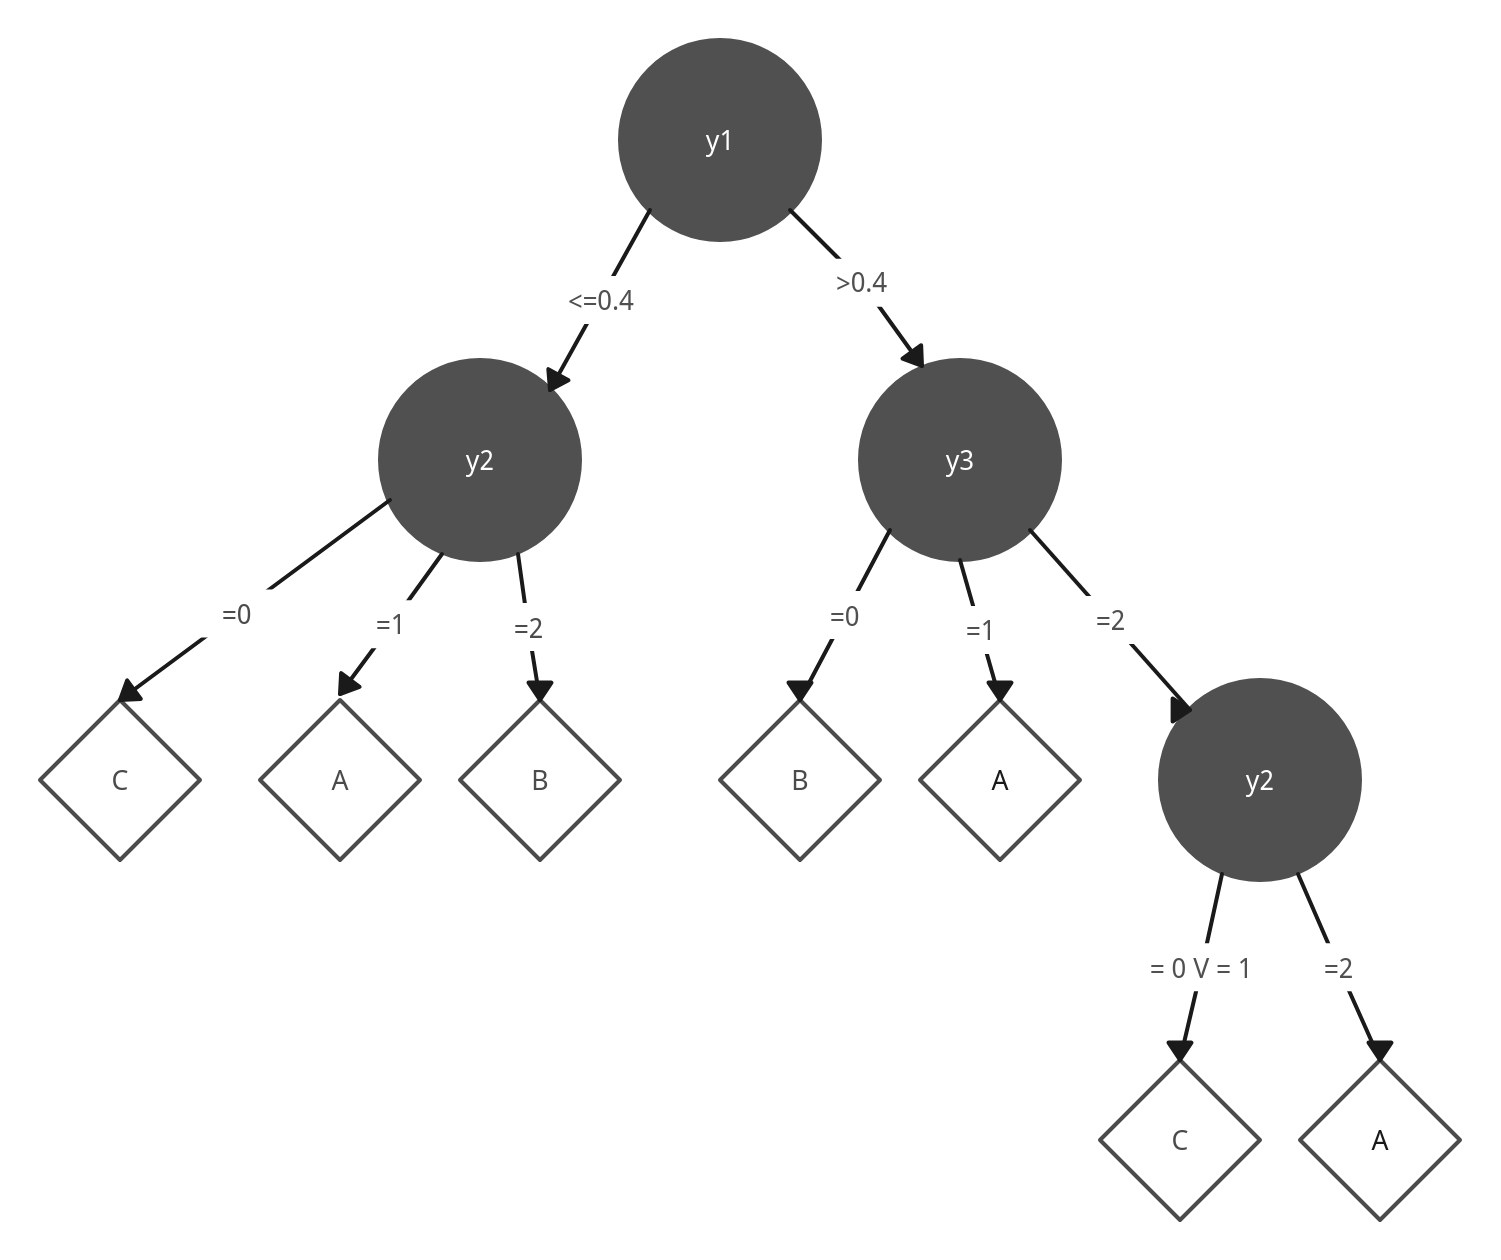
\includegraphics[width=14cm]{./assets/decision_tree_ex1_PartI.png}
        \caption{Decision Tree for exercise I.1}
        \label{fig:decision_tree}
    \end{figure}

    \item \textbf{Draw the training confusion matrix for the learnt decision tree.}

    \vskip 0.3cm
    Following the learnt decision tree above, we can predict the values for each observation.
    For each observation, we look at the value for the first variable ($y_1$) and follow the branch that corresponds with its value.
    From the node we arrive at, we do the same thing for the next variable, and we keep doing this until we reach a leaf.
    The class present in this leaf will be the predicted value, while the real value is the value of $y_{out}$ for that observation.
    Below we present the real values along with the predicted ones:

    \begin{center}
        \begin{tabular}{cccccccccccccc}
            \multicolumn{2}{c}{}           & $x_1$ & $x_2$ & $x_3$ & $x_4$ & $x_5$ & $x_6$ & $x_7$ & $x_8$ & $x_9$ & $x_{10}$ & $x_{11}$ & $x_{12}$ \\
            \multirow{1}{*}{real}      & = & [A   & B   & B   & C   & C   & A   & A   & A   & B   & B   & C   & C] \\
            \multirow{1}{*}{predicted} & = & [A   & B   & C   & C   & C   & A   & A   & A   & A   & B   & C   & C]
        \end{tabular}
    \end{center}

    \textbf{Finally}, we can show the count of each pair of real and predicted values in a confusion matrix (e.g. 4 pairs of AA from observations $x_1$, $x_6$, $x_7$, $x_8$):

    \vspace{0.5em}
    \begin{center}
        \begin{tabular}{|c|c|c|c|c|c|}
            \cline{3-5}
            \multicolumn{2}{c}{}                & \multicolumn{3}{|c|}{\textbf{Real}} & \multicolumn{1}{c}{} \\
            \cline{3-5}
            \multicolumn{2}{c|}{}               & \textbf{A} & \textbf{B} & \textbf{C} & \multicolumn{1}{c}{} \\
            \hline
                                                & \textbf{A} & 4 & 1 & 0 & 5 \\
            \cline{2-6}
            \multirow{1}{*}{\textbf{Predicted}} & \textbf{B} & 0 & 2 & 0 & 2 \\
            \cline{2-6}
                                                & \textbf{C} & 0 & 1 & 4 & 5 \\
            \hline
            \multicolumn{2}{c|}{}               & 4 & 4 & 4 & 12 \\
            \cline{3-6}
        \end{tabular}
    \end{center}

    \item \textbf{Identify which class has the lowest training F1 score.}

    \vskip 0.3cm

    \(F1_{score}\) is given by the following equation:

    \begin{equation}\label{ex3-f1}
        F1_{score} = 2 \cdot \frac{{\text{precision} \cdot \text{recall}}}{{\text{precision} + \text{recall}}}
    \end{equation}

    And precision and recall are given by:

    \begin{equation}\label{e3-p}
        \text{Precision} = \frac{\text{True Positives}}{{\text{True Positives} + \text{False Positives}}}
    \end{equation}

    \begin{equation}\label{e3-r}
        \text{Recall} = \frac{\text{True Positives}}{{\text{True Positives} + \text{False Negatives}}}
    \end{equation}

    Therefore, \textbf{let's start by calculating the precision for A, B and C} by replacing the values on \eqref{e3-p}:

    \[
        \begin{aligned}
            Precision_A = \frac{4}{4+1} = \frac{4}{5}
        \end{aligned}
    \]

    \[
        \begin{aligned}
            Precision_B = \frac{2}{2+0} = 1
        \end{aligned}
    \]

    \[
        \begin{aligned}
            Precision_C = \frac{4}{4+1} = \frac{4}{5}
        \end{aligned}
    \]


    \textbf{Now, it's time to calculate the recalls for A, B and C}, using the equation on \eqref{e3-r}:

    \[
        \begin{aligned}
            Recall_A = \frac{4}{4+0} = 1
        \end{aligned}
    \]

    \[
        \begin{aligned}
            Recall_B = \frac{2}{2+2} = \frac{1}{2}
        \end{aligned}
    \]

    \[
        \begin{aligned}
            Recall_C = \frac{4}{4+0} = 1
        \end{aligned}
    \]

    \textbf{Finally, let's calculate the $F1_{score}$}, using the equation \eqref{ex3-f1}:

    \[
        \begin{aligned}
            F1_{score} A = 2 \cdot \frac{{ \frac{4}{5} \cdot 1 }}{{ \frac{4}{5} + 1 }} = 0.8889
        \end{aligned}
    \]

    \[
        \begin{aligned}
            F1_{score} B = 2 \cdot \frac{{ \frac{1}{2} \cdot 1 }}{{ \frac{1}{2} + 1 }} = 0.6667
        \end{aligned}
    \]

    \[
        \begin{aligned}
            F1_{score} C = 2 \cdot \frac{{ 1 \cdot \frac{4}{5} }}{{ 1 + \frac{4}{5} }} = 0,8889
        \end{aligned}
    \]

    \textbf{The class with the lowest training score is B}, with a score of 0.6667.

    %\textbf{VERIFICAR ISTO EM CASA (pdf e resultado). TODO}

    \item \textbf{Considering $y_2$ to be ordinal, assess if $y_1$ and $y_2$ are correlated using the Spearman coefficient.}

    \vskip 0.3cm

    To calculate the Spearman coefficient when there's rank, we have to use the following equation:

    \begin{equation}\label{ex4-sp}
        \begin{split}
            \text{Spearman}(y_x, y_y) = \frac{\text{cov}(y_x, y_y)}{\sigma_{y_x} \sigma_{y_y}}
            = \frac{\sum_{i=1}^{n} (x_i - y_x)(y_i - y_y)}{\sqrt{\sum_{i=1}^{n} (x_i- \bar{y_x})}\sqrt{\sum_{i=1}^{n} (y_i- \bar{y_y})}}
        \end{split}
    \end{equation}

    Firstly, \textbf{let's order $y_1$ and $y_2$} so we can calulate the ranks and $y'_1$ and $y'_2$:

    \begin{align*}
        ordered\_y_{1} & = [0.04, 0.06, 0.24, 0.32, 0.36, 0.44, 0.46, 0.52, 0.62, 0.68, 0.76, 0.9]\\
        ranks\_y_{1}   & = [1,2,3,4,5,6,7,8,9,10,11,12]\\
        y'_{1}         & = [3,2,1,5,4,10,12,11,7,9,6,8]\\
        ordered\_y_{2} & = [0,0,0,0,0,0,1,1,1,2,2,2]\\
        ranks\_y_{2}   & = [3.5, 3.5, 3.5, 3.5, 3.5, 3.5, 8, 8, 8, 11, 11, 11]\\
        y'_{2}         & = [8, 11, 3.5, 3.5, 3.5, 11, 3.5, 11, 8, 3.5, 8, 3.5]
    \end{align*}

    Now, we have all we need to calculate \textbf{the Spearman coefficient} using the expression at \eqref{ex4-sp}. Here is the result:

    \[
        Spearman(y_{1}, y_{2}) = 0.07966
    \]

    %\textbf{VALOR A CONFIRMAR EM CASA (pdf e resultado). TODO}

    \item \textbf{Draw the class-conditional relative histograms of $y_1$ using 5 equally spaced bins in $[0,1]$.
    Find the root split using the discriminant rules from these empirical distributions.}

    \vskip 0.3cm
    Blah
\end{enumerate}

\vskip 0.5cm

\begin{center}
\large{\textbf{Part II}: Programming}\normalsize
\end{center}

\noindent Consider the \texttt{column\_diagnosis.arff} data available at the homework tab, comprising 6 biomechanical
features to classify 310 orthopaedic patients into 3 classes (\texttt{normal}, \texttt{disk hernia}, \texttt{spondilolysthesis}).

\begin{enumerate}[leftmargin=\labelsep]
    \item \textbf{Apply \texttt{f\_classif} from \texttt{sklearn} to assess the discriminative power of the input variables.
          Identify the input variable with the highest and lowest discriminative power.
          Plot the class-conditional probability density functions of these two input variables.}

          \vskip 0.3cm
          \lstinputlisting[language=Python]{./assets/code_1.py}

          As you can see in the graph ahead, the highest discriminative power variable is \textit{degree\_spondilolysthesis} and
          the lowest discriminative power variable is \textit{pelvic\_radius}.

          \vskip -0.57cm

          \begin{figure}[H]
              \centering
              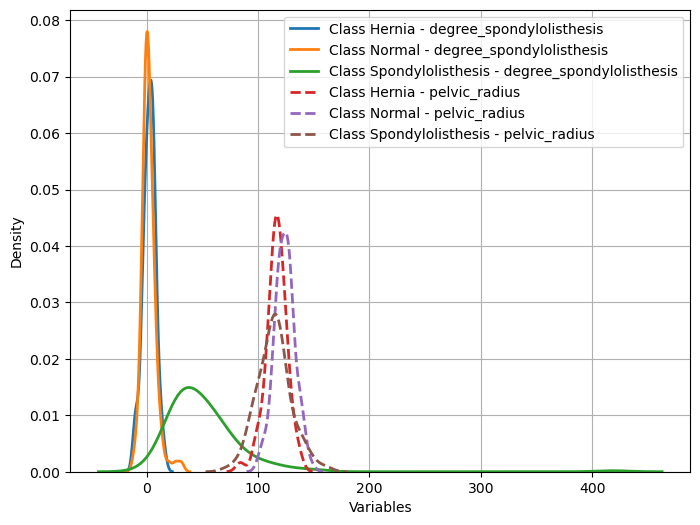
\includegraphics[width=14cm]{./assets/class_conditional_probability.png}
              \caption{Class-conditional probability density functions of the highest and lowest discriminative power variables.}
              \label{fig:PartII-ex1-plot}
          \end{figure}

    \item \textbf{Using a stratified 70-30 training-testing split with a fixed seed (\texttt{random\_state=0}), assess in a
          single plot both the training and testing accuracies of a decision tree with depth limits in
          $\{1,2,3,4,5,6,8,10\}$ and the remaining parameters as default.\vskip 0.05cm
          \textit{[Optional]} Note that split thresholding of numeric variables in decision trees is non-deterministic
          in sklearn, hence you may opt to average the results using 10 runs per parameterization.}

          \vskip 0.3cm
          \lstinputlisting[language=Python]{./assets/code_2.py}

          \vskip -0.7cm
          \begin{figure}[H]
              \centering
              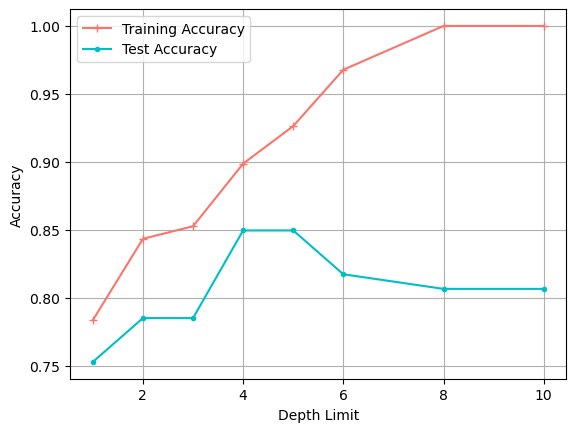
\includegraphics[width=14cm]{./assets/training_testing_accuracies.png}
              \caption{Accuracy of the trained decision tree, applied to both a test and training sets, for varying depth limits.}
              \label{fig:PartII-ex2-plot}
          \end{figure}

    \item \textbf{Comment on the results, including the generalization capacity across settings.}

          \vskip 0.3cm
          % Depth Limit and Training Accuracy
          The graphic illustrates that as the depth limit of the decision tree increases, the training accuracy steadily rises.
          This observation suggests that deeper trees can better fit the training data, capturing intricate patterns and achieving higher accuracy when evaluated
          on the same dataset. However, it's crucial to keep in mind that higher training accuracy doesn't necessarily translate to better predictive
          performance on unseen data.

          % Generalization Capacity
          The testing accuracy follows a distinct pattern. Initially, it improves as the depth limit
          increases, indicating improved generalization. However, beyond a certain depth limit (around 4 or 5 in this case), the testing accuracy starts to
          decline. This signifies a loss in generalization capacity, a phenomenon known as overfitting. It implies that overly complex decision trees can fit
          noise in the training data and perform poorly on new, unseen data.

          % Optimal Depth Limit
          The optimal depth limit appears to be around 4 or 5, striking a balance between model complexity and generalization to new data.
          It's crucial to avoid both underfitting (too simple) and overfitting (too complex) by selecting a depth limit that maximizes testing accuracy.
          \vskip 0.3cm

    \item \textbf{To deploy the predictor, a healthcare team opted to learn a single decision tree
          (\texttt{random\_state=0}) using \textit{all} available data as training data, and further ensuring that each leaf has
          a minimum of 20 individuals in order to avoid overfitting risks.}
          \begin{enumerate}
          \item \textbf{Plot the decision tree.}

          \vskip 0.3cm
          \lstinputlisting[language=Python]{./assets/code_4_a.py}

          \vskip -0.7cm
          \begin{figure}[H]
              \centering
              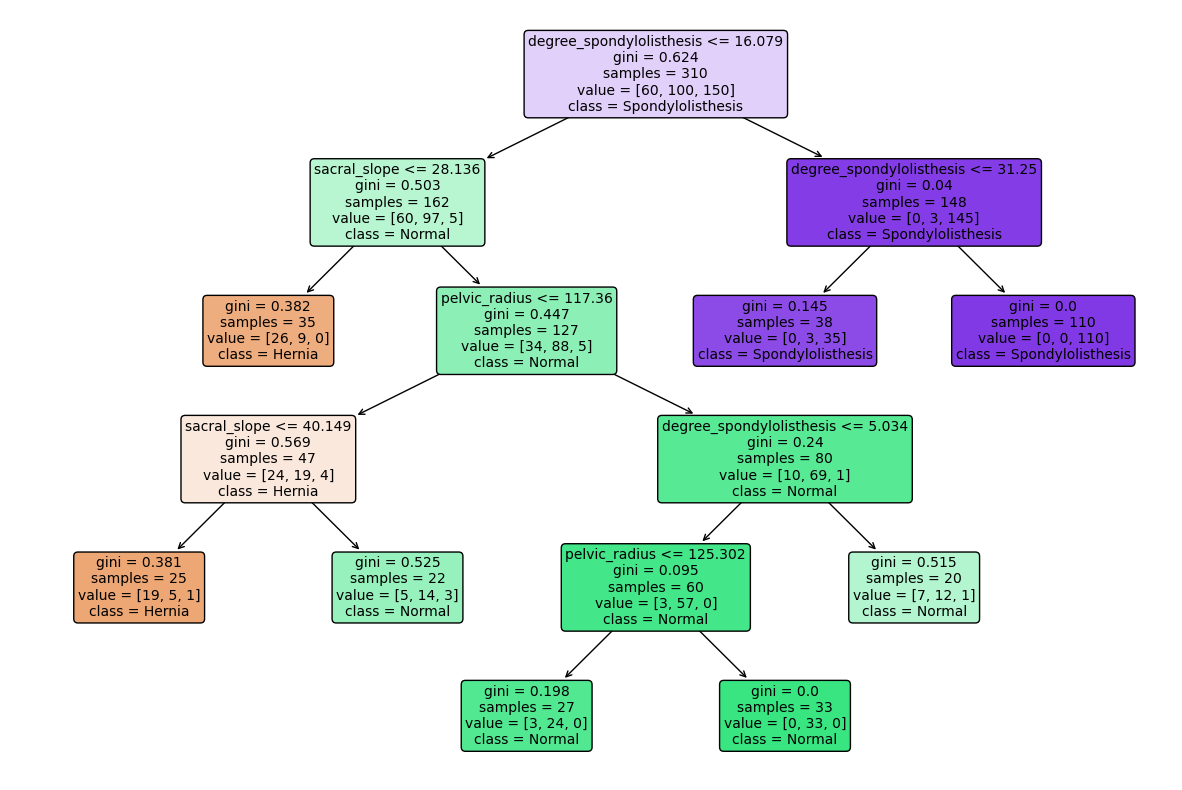
\includegraphics[width=\linewidth]{./assets/decision_tree_ex4a_PartII.png}
              \caption{Decision Tree for exercise II.4a}
              \label{fig:PartII-ex4a-plot}
          \end{figure}

          \item \textbf{Characterize a hernia condition by identifying the hernia-conditional associations.}

          \vskip 0.3cm

          The hernia condition can be characterized by:
          \begin{enumerate}
            \item Spondilolysthesis degree $\leq 16.079$, sacral slope $\leq 28.136$
            \item Spondilolysthesis degree $\leq 16.079$, sacral slope $\leq 28.136$, and pelvic radius $\leq 117.36$
          \end{enumerate}
          \end{enumerate}
\end{enumerate}

\vskip 1cm
\center\textbf{END}

\end{document}
